\section{Input}

\subsection{Medium Selection}
\label{sec:medium-selection}

The first step in this project was to establish the best method for a student to interact with the application. As seen in \cref{sec:prior-research} a lot of different mediums for OMR have been tried over the years, however which one would be most suitable for a student to use wouldn't necessarily correlate with which was best for quality of scanning, speed of analysis etc.

\subsubsection{Flat Bed Scanner}

The most simple of all the input methods, this would involve a student writing on a sheet of manuscript paper, then using a flat bed scanner (the type commonly found as a standalone device and in multi-function printers) to input the sheet into the computer. This method allows for a scan with high and consistent light levels (minimising noise and light-dependent artefacts), minimal distortion due to paper curvature (as the scanner usually flattens the sheet) and a high resolution end image, typically 300-600dpi.

The application would process the sheet using traditional OMR techniques and then provide feedback to the student. This technique would therefore require ownership of both a scanner and a computer on which to install and run the application. Alternatively, the student could upload the scanned image to a web based service for analysis, removing the need to install software.

\subsubsection{Photograph/Camera}

\todo[inline,color=red]{Implementation - Photo/Camera}

Total free for all, colours and light levels vary, extraction from background, resolution variable, noise variable

Reference `Project 8 Final Report'

\subsubsection{Gestures}
\todo[inline,color=red]{Implementation - Gestures}

Use gestures combined with classification (see book and some papers).
Good for classifying individual entities but more like the old palm tablets, usually one note at a time

\subsubsection{Tablet Input}
\todo[inline,color=red]{Implementation - Tablet Input}

Finger or stylus work well tends to depend on the child, finger often felt more natural

\begin{figure}[h!]
    \centering
    \begin{subfigure}[b]{.49\linewidth}
        \centering
        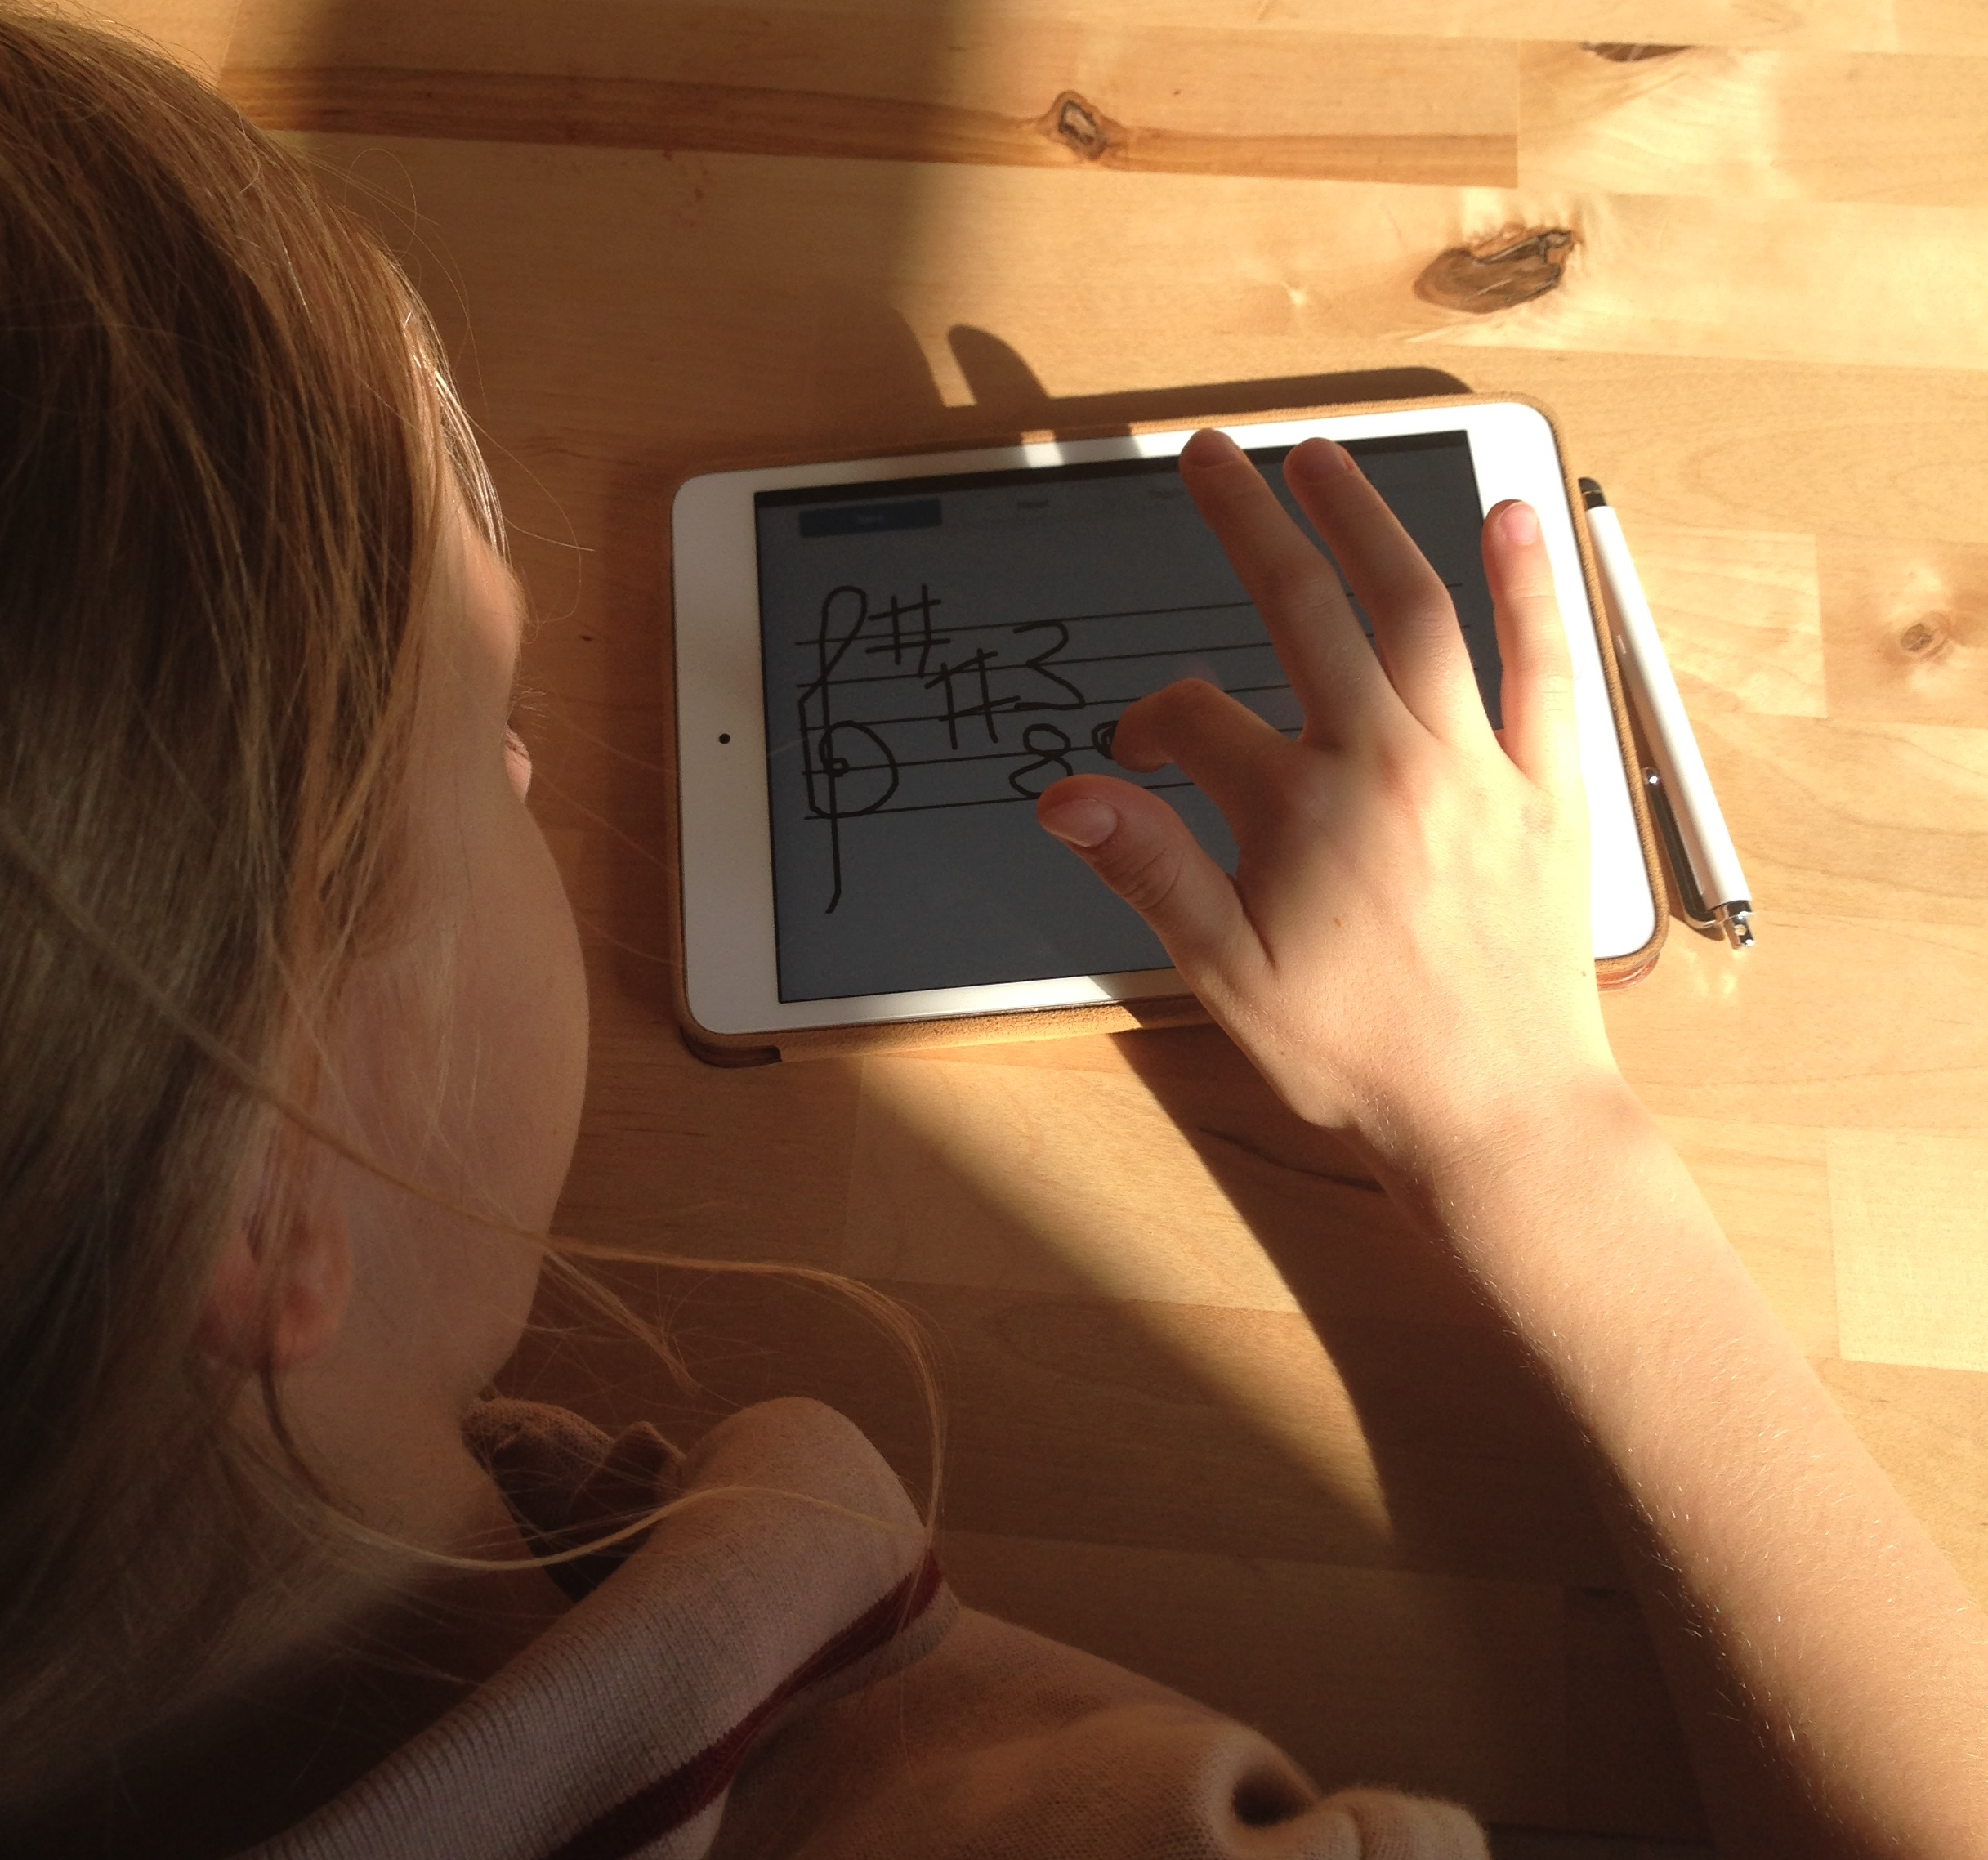
\includegraphics[width=\linewidth]{gfx/photos/user-finger.jpg}
        \caption{Using a finger}
    \end{subfigure}
    \begin{subfigure}[b]{.49\linewidth}
        \centering
        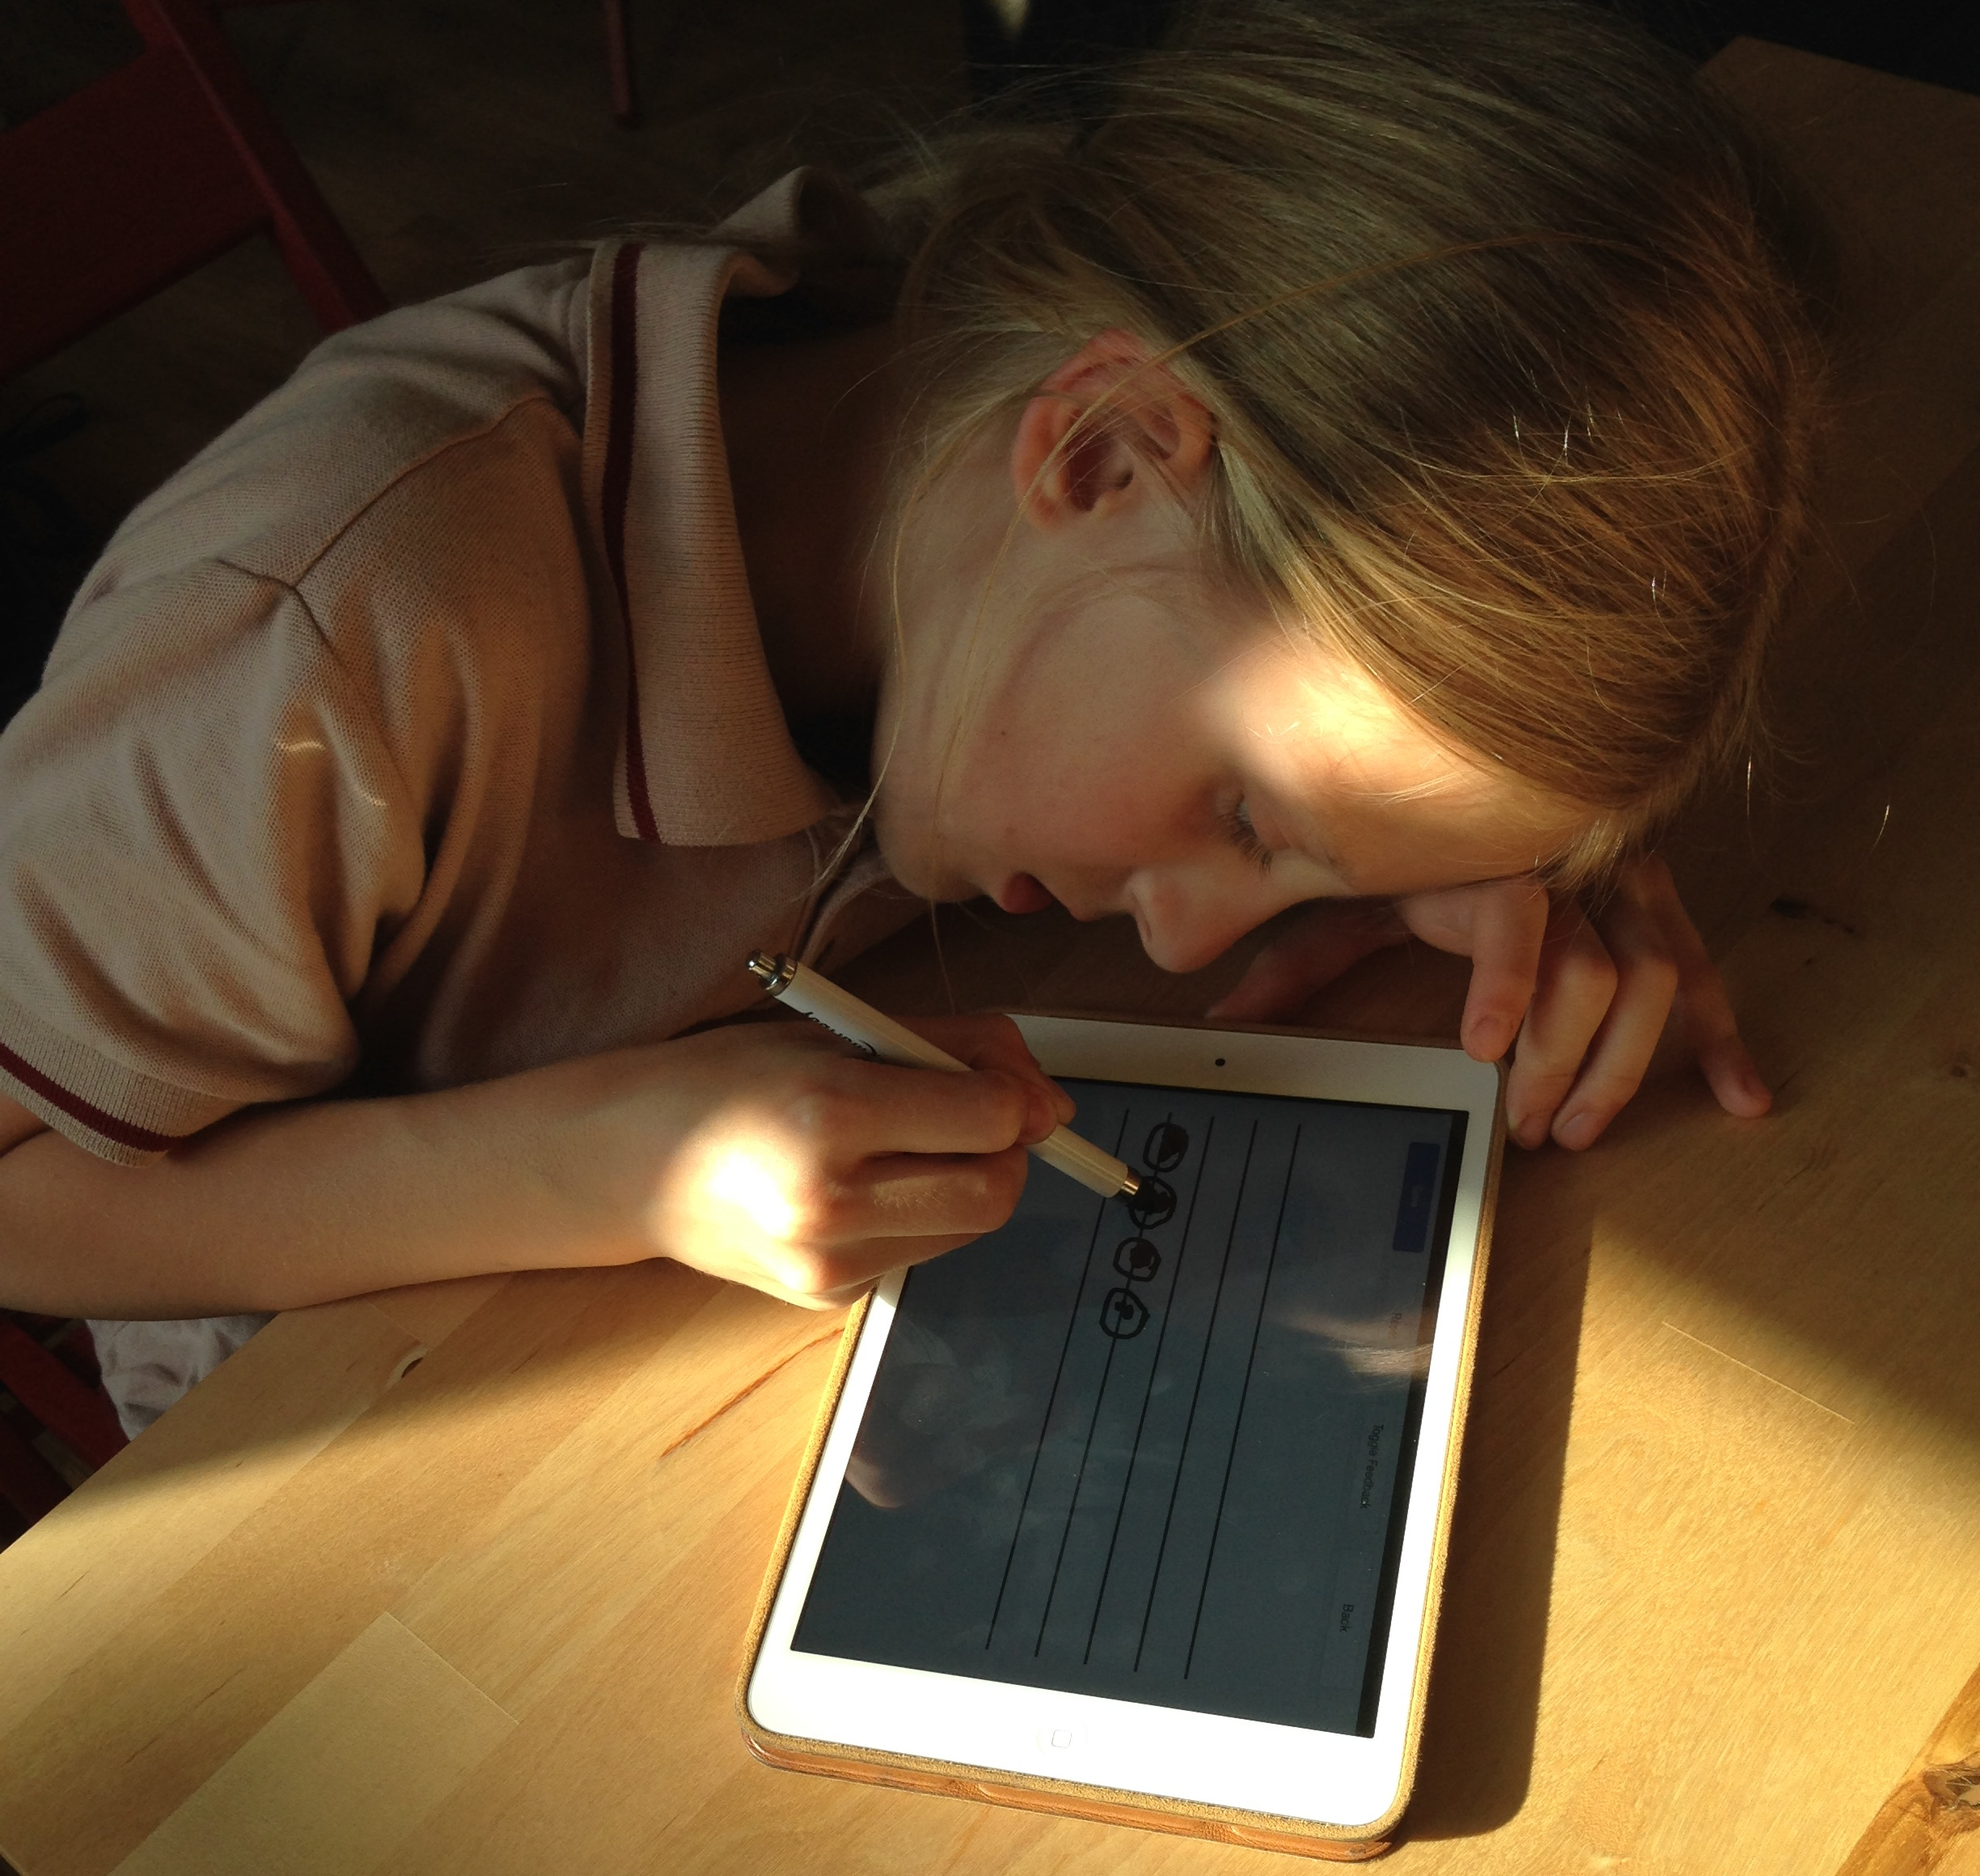
\includegraphics[width=\linewidth]{gfx/photos/user-stylus.jpg}
        \caption{Using a stylus}
    \end{subfigure}

    \caption{Examples of a student trying different tablet input methods}
\end{figure}

Chose this method in the end


\subsection{Capturing Strokes}
\label{sec:capturing-strokes}
To capture strokes drawn by the user, several listeners are attached to the HTML5 canvas element on which the manuscript is rendered. When the user presses their mouse down or initiates a touch event, a new array of line points is created and the initial point of interaction is stored in that array. From there, any mouse or touch movement whilst the touch or `mousedown' event is active triggers a new point recording, until the mouse button is released or the touch event ends. In this way, an array of points is built up which represent a drawn line.

Each time the line changes via the addition of new points, a redraw event is triggered which connects all the points together and renders the line onto the canvas.

In initial experiments with simple manuscript entities, this worked well, however as children began to experiment with more complex entities (requiring more lines and therefore more points) the length of time required to redraw the lines on the canvas became prohibitively long. Eventually a lag occurred between `pen' movement and lines being rendering on the canvas, the result of which was that as more lines were drawn, the time between new points being registered increased. This increase led to the drawing experience feeling (as one user described it) `really clunky' and long straight lines appearing instead of smooth curves (\cref{fig:drawing-lag-rough}).

\begin{figure}[hbt                                   ]
    \centering

    \begin{subfigure}[b]{.49\linewidth}
        \centering
      
\includegraphics[width=\linewidth]{gfx/implementation/lag-stave.png}
      \caption{Drawing with refresh rendering - note that after drawing a high density region of many points, a spiral outward is very `angular' due to the additional time it takes to redraw so many points on every movement event }
      \label{fig:drawing-lag-rough}
    \end{subfigure}
    \begin{subfigure}[b]{.49\linewidth}
        \centering
      
\includegraphics[width=\linewidth]{gfx/implementation/nolag-stave.png}
      \caption{Drawing with incremental rendering, not that after a similar high density region of points, the curve outwards still appears smooth}
      \label{fig:drawing-lag-smooth}
    \end{subfigure}
    
  \label{Drawing Lag}
    
\end{figure}

To counteract this, I modified the code such that it renders new line segments on the fly, rather than re-rendering all the lines every time a new point is added. Although this requires some more logic to render the line segment, this was more than compensated for by the increase in the smoothness of the drawing experience and the resulting image (\cref{fig:drawing-lag-smooth}).

\section{Data Storage and Retrieval}

\subsubsection{Stave Drawing}
Initially I planned to store the data gathered in \cref{sec:capturing-strokes} as serialized JSON in the database. When image processing was required, I could then simply re-render the canvas server-side when performing the various image processing techniques outlined in \cref{sec:techniques}. However, after some initial experimentation I felt that sending the canvas data directly to the server as a compressed blob exactly as it was rendered in the browser was a better implementation.

Firstly, there is no better representation of the user's drawing than a precise pixel for pixel representation. However I re-render the lines server-side, making the output exactly mirror that of the user's drawing would be hard to get right.

Also, since the image processing techniques I employ require actual image data as opposed to lines and points, we don't have to re-render the drawing every time image processing is required, we can simply load the data directly from the database.

Finally, since the user interface involves showing previous drawings to the user, streaming the captured canvas directly from disk eliminates another section of the application which would require re-rendering of the image.

\todo[inline]{Should I show my database schema here?}

\subsubsection{Components}

Once components have been extracted from the drawing using the techniques outlined in \cref{sec:identification}, I store both their features and \acrfull{RLE} representation of the whole component in the database for retrieval later during any further image processing.

Although 3000 components uses around 1GB in data when raw, using compression we are able to lower this considerably as shown in \ref{sec:identification-rle}.


